The current implementation consists of two independent parts. The weather collector component which is described in \cref{subsec:weather} is developed with  NodeJS express. The main component which handles all the simulation and calculations is written in Java and uses the Spring Boot framework. The theoretical foundation of this component is described in \cref{subsec:Windturbine} and the following. Both components are linked through a shared database.

\subsection{Gather weather design}\label{subsec:weather}
\subsubsection{Weather service}\label{sec:weatherservice}
For our smart energy system, we need a weather service which can provide all needed data on an hourly basis.
There is one weather service which fulfills our needs more than appropriate.
The weather service \url{weatherbit.io} has different kinds of endpoints on its API.
In our case we use two of them, the current weather data API and the 48 hours weather forecast API.

Before we take a look at the endpoints provided to the user and their responses, we want to present the data collectable on weatherbit.io.
An example response of the current weather API is shown in listing \ref{lst:weatherdata}.
The property  \texttt{data} of the JSON object contains an array of weather data points.
For current weather API there is only one object in the array.
But for the forecast there are up to 48 objects, one for every hour of the forecast.
\begin{lstlisting}[caption={Example response of weatherbit.io for $lat=31.23$ and $lon=121.47$}, label={lst:weatherdata}, frame=single, language=json]
 {
    "data": [
        {
            "wind_cdir": "SSE",
            "rh": 100,
            "pod": "n",
            "lon": 121.47,
            "pres": 1012.2,
            "timezone": "Asia/Shanghai",
            "ob_time": "2018-11-07 20:35",
            "country_code": "CN",
            "clouds": 0,
            "vis": 10,
            "solar_rad": 0,
            "state_code": "23",
            "wind_spd": 0.89,
            "lat": 31.23,
            "wind_cdir_full": "south-southeast",
            "slp": 1013.2,
            "datetime": "2018-11-07:20",
            "ts": 1541622900,
            "station": "E7205",
            "h_angle": -90,
            "dewpt": 13.9,
            "uv": 0,
            "dni": 0,
            "wind_dir": 156,
            "elev_angle": -29.2797,
            "ghi": 0,
            "dhi": 0,
            "precip": null,
            "city_name": "Shanghai",
            "weather": {
                "icon": "c01n",
                "code": "800",
                "description": "Clear sky"
            },
            "sunset": "09:00",
            "temp": 13.9,
            "sunrise": "22:14",
            "app_temp": 13.9
        }
    ],
    "count": 1
}
\end{lstlisting}
From all those data we chose only to store \texttt{lat} for latitute, \texttt{lon} for longitute, \texttt{pres} for air pressure, \texttt{rh} for relative humidity, \texttt{ghi} for global horizontal solar irradiance, \texttt{wind\_spd} for wind speed, \texttt{temp} for the temperature, and the timestamp in UTC format.

The API for the current weather data returns current weather data of over 45.000 stations.
Every API request will return the nearest, and most recent observation.
There are several endpoints available in the API.
For example, a user can get current weather observation by lat/lon as we do or by city name.
All endpoints differ only on their required query parameters.
They define whether to get the observation by lat/lon, city name or any other possible way.
The basepath for all endpoints is \texttt{https://api.weatherbit.io/v2.0/current} and the supported method is \texttt{GET}.
To get the data in the metric format you have to add an additional query parameter \texttt{unit=m}.
Every request must provide an API key in query parameters.\cite{weatherbit}
This API key can be requested by creating an account on weatherbit.io.
After creating an account a user has to choose a pricing plan.
For our system the free plan is totally sufficient.

The API for the weather forecast data returns the weather forecast for up to 48 hours on an hourly basis.
Nevertheless, we only request it for 24 hours.
While the basepath is now \texttt{https://api.weatherbit.io/v2.0/forecast/hourly}, the provided query parameter are the same with an additional query parameter \texttt{hours} which must get a value between 0 and 48 to specify the size of the forecast.

\subsubsection{Our WeatherCollector service}\label{sec:weathercollector}
To gather weather data for different locations and store it into a database we build a service, which is under MIT licence available on GitHub\footnote{\url{https://github.com/smart-energy-system/WeatherCollector}}.
The service runs a NodeJS express server with two endpoints to create or delete \texttt{WeatherCollector} objects. 
A \texttt{WeatherCollector} object gathers every hour current weather data for a given location as well as 24 hours weather forecast on an hourly basis and stores the data in a database. 
While gathering new forecast data, the old deprecated data is getting replaced, so there is always the latest 24 hour forecast data. Multiple WeatherCollector objects are possible to collect weather data for different locations at the same time.

There are several dependencies you have to install before running the server. 
Since the code runs on NodeJS version 8 or higher with a current npm, you need to have this installed first.
First, run \texttt{npm install} to install needed dependency packages. 
You can look up the installed libraries and their versions in \texttt{package.json} file. 
After installing the packages, you need to create the database. 
Therefore, run \texttt{node DBCreator.js} to create the database file and required SQL tables. 
Now you are nearly ready to run the server.

You can test the functionality without running the complete server.
You just need to run \texttt{WeatherCollectorTest.js} to play around with some locations. 
On the first run of the module you need to provide it with your weatherbit.io API key, latitute and longitute of the location: \texttt{node WeatherCollectorTest.js "<API Key>" <lat> <lon> "<mode>"}. 
Keep in mind that you already need the API key requested from weatherbit.io.
There are 5 modes available to test:
\begin{itemize}
	\item \texttt{collect}: Collects a current weather data of the given location and stores it into the database
	\item \texttt{get}: Gets the latest stored current weather data of the given location
	\item \texttt{collect forecast}: Collects a 24 hour weather forecast on hourly basis for a given location and stores it into the database
	\item \texttt{get forecast}: Gets the latest version of the forecast weather data of the given location
	\item \texttt{start}: Starts a WeatherCollector object on hourly picking new weather data (current and forecast) and stores the data into the database.
\end{itemize}

If you did run the complete run command once, a test config file was created. 
So unless you want to change your API key or the location you can shorten the run command a bit, using only \texttt{node WeatherCollectorTest.js "<mode>"}.

You can simply run the server with \texttt{npm start <API key>}. 
This will create a config file with your API key, so later you can start the server just running \texttt{npm start} command.

Since the service is a REST service, there are two HTTP REST endpoints available on the server, one for creating WeatherCollector objects and one for deleting them.
To create a new WeatherCollector object, you can send an \texttt{POST} request against \texttt{<basepath>/weathercollectors} providing the body shown in listing \ref{lst:postbody} as content-type \texttt{application/json}. 
\begin{lstlisting}[caption={Body of \texttt{POST} request endpoint}, label={lst:postbody}, frame=single, language=json]
{ 
	"lat":<lat>, 
	"lon": <lon> 
}
\end{lstlisting} 
If \texttt{lat} and \texttt{lon} are correct and the object is created successfully you will get status 201 and a JSON object as shown in listing \ref{lst:postresponse} in return.
\begin{lstlisting}[caption={Body of the response of the \texttt{POST} request}, label={lst:postresponse}, frame=single, language=json]
{ 
	"lat": <lat>, 
	"lon":<lon>, 
	"id":<id> 
}
\end{lstlisting}
The \texttt{id} is the ID of the object created. 
You will need it to delete the object later, so better save it anywhere. 
After creating the object, the object is requesting the weather data (current and forecast) every hour. 
If one of the request body properties is not defined you will get a status 400 in return.

To delete a WeatherCollector object of given ID, you can send an \texttt{DELETE} request against \texttt{<basepath>/weathercollectors} providing the in body the data shown in listing \ref{lst:deletebody} as content-type \texttt{application/json}.
\begin{lstlisting}[caption={Body of \texttt{DELETE} request endpoint}, label={lst:deletebody}, frame=single, language=json]
{ 
	"id":<id> 
}
\end{lstlisting}
If \texttt{id} is set and there is a WeatherCollector object with such an ID, it will be deleted and therefore stops gathering data. 
The return will be status 200. 
If id is not set or there is no WeatherCollector object with such an ID, the return will be status 400.




\subsection{Windturbine}\label{subsec:Windturbine}
\subsubsection{Swept area function}
The swept area of a wind turbine is dependent on the radius of the rotary blades. Combined with the constant Pi the area swept can be computed by the equation\cite{Beckmann}: $A = r^{2}* \Pi  $
\subsubsection{Vapor pressure}
To compute the actual vapor pressure in the air the relative humidity has to be given. The relative humidity is computable with the equation $H = P_{av} / P_s$ with $P_{av}$ being the actual vapor pressure and $P_s$ being the saturated vapor pressure at a given temperature. This equation can be restructured to get the actual vapor pressure: $P_{av}  = H * P_s$. The relative humidity is a parameter for the function, which is filled with data from the before mentioned weather data collection.\\
\\
To be able to now compute the actual vapor pressure at a given temperature we still need the saturated vapor pressure. For this we can use the Herman Wobus equation (E being the vapor pressure):\\
$E = e/p^{8}$ with\\
e = 6.1078 and\\
$p = c_0 + T * (c_1 + T * (c_2 + T * (c_3 + T * (c_4 + T *(c_5 + T * (c_6 + T * (c_7 + T * c_8 + T * c_9)))))))$\\
with $c_0$ to $c_9$ being constants and T being the temperature in degrees Celsius.\cite{AirDensity,NOAA}
\subsubsection{Density of moist air}
In order to compute the density of moist air, we have to have a look at how it is compounded. Moist air density is a mixture of dry air and water vapor. The physical equation for this is: $D_m = (P_d/(R_d * T_k))+(P_v/(R_v*T_k))$\\
$D_m$ is the density of moist air, $P_d$ is the pressure of dry air at the specified temperature, $R_d$ is the gas constant for dry air, $P_v$ is the pressure of water vapor at the specified temperature, $R_v$ is the gas constant for water vapor and $T_k$ is the given temperature in degrees Kelvin. With the previously implemented methods this equation system is able to compute the air density with only the temperature and relative humidity given.\cite{AirDensity,Shelquist}
\subsubsection{Wind turbine model}
The wind turbine model contains some variables which can be set by the user. The function for computing the generated energy is derived from the power coefficient of the turbine (basically the efficiency), the size of the turbine (shows in area swept), the density of the air in the area and of course the weather conditions which apply at the moment given.
The general equation for this setup is: $P_{avail} = (1/2) * p * A * v^{3} * C$
where p is the air pressure, A the area swept, v the windspeed and C the power coefficient. \cite{WindPowerCalcs}
\subsection{Photovoltaic}
\subsubsection{Temperature loss}
The function for the temperature loss is giving a linear function for the percentage loss of energy depending on the degrees over 25 degree Celsius. We made the assumption that the efficiency does not go over 100 \% even for temperatures below 25 degree Celsius.The resulting equation is as follows: $L_t = max((T-25)*0.005 , 0)$ with the result being the percentage of energy lost due to temperature as a point number.
\subsubsection{Performance ratio}
The performance ratio is sum of all losses.
With the previous computed losses for temperature and the constant loss $L_0$ of 0.14 we get the equation $R = (L_0 + L_t) = 1.0 - (0.14 + L_t)$. To use  the result in our calculation we have to subtract the result form 1.
\subsubsection{Solar irradiance}
The computation of the solar radiation incident and therefore the effective solar radiation on the surface of the solar panel can be computed with the equation $(SP_{horizontal} * sin(\alpha + \beta))/sin(\alpha)$.
$\alpha$ is the effective tilt of solar radiation on a specified latitude and set as $90 - latitude$ of the position from the solar panel + $\delta$.
$\delta$ is the tilt of the solar radiation in regard of the day of the year d and can be computed with the following equation: $23.45 * sin((360/365) * (284 + d))$. $(SP_{horizontal}$ is the horizontal solar radiation. Our weather service provides us with this information.
The tilt of the solar panel  itself is used as $\beta$. \cite{SolarRadiation}
\subsubsection{Photovoltaic model}
The formula for computing the generated energy as given in the slides is: $E = A * r * PR * S$\\
A is the area of the solar panel and is given by the user in $m^{2}$.
Same goes for the solar panel yield r which is given by the user via the maximum power yield as well.
The performance ratio PR  is computed in on of the previous steps and is  a percentage.
S is the solar radiation incident and is computed in regards of solar radiation and other factors taken from the database.
The measurement unit for S is $W/m^{2}$.
The resulting unit for produced energy is therefore W.
\subsubsection{Battery model}
The first function for returning the current state of the battery is a simple return of the currently stored energy.
The formula for charging and discharging is more complex and takes several parameters.
The parameters are charging and discharging rate as well as charging efficiency.
The function returns the actual change of energy stored in the battery.
The returned value is positive if the battery is charged and negative if the battery is discharged.
\subsubsection{Demand profile}\label{subsec:Demand}

Our demand profile is based on data from \texttt{\url{https://open-power-system-data.org/}}. We use the \glqq{}Household Data\grqq{} package from 2017-11-10. The calculations are based on the 60 minutes interval data set. We use two different profiles, one is based on the feed \textit{DE\_KN\_residential2 \_grid\_import} and the other is based on \textit{DE\_KN\_industrial3\_grid\_import}. The raw data from Open Power System Data always report the total amount of energy used so far in kWh. Based on this we needed to calculate the difference between the data points to the get change of the total value per hour. After that, we calculated the average value for each hour of the day for all data points. The consumer in profile 1 used in total about 4500 kWh in the time between the 15. April 2015 and the 1. February 2017. This equals roughly a total of 2500 kWh per year. The second consumer used in total 695000 kWh in the time between 11. February 2016 and 09. February 2017. Our electricity provider estimates a small one or two people household for the first consumer based on the total usage per year \cite{enbw}. Based on this we amused a floor area size of 50 $m^{2}$. \Cref{fig:profile1} and \cref{fig:profile2} visualize the demand profiles. The user does not only provide an area but also an average daily occupancy. We assumed that the latter value is the fraction of the time in which the building is in use. Based on this we calculate the final energy demand D for each hour for a building with this formula $ D = profileDemandPerSquareMeter_{hourOfTheDay} * floorAreaSize * averageDailyOccupancy$. 

\begin{figure}[!h]
	\centering
	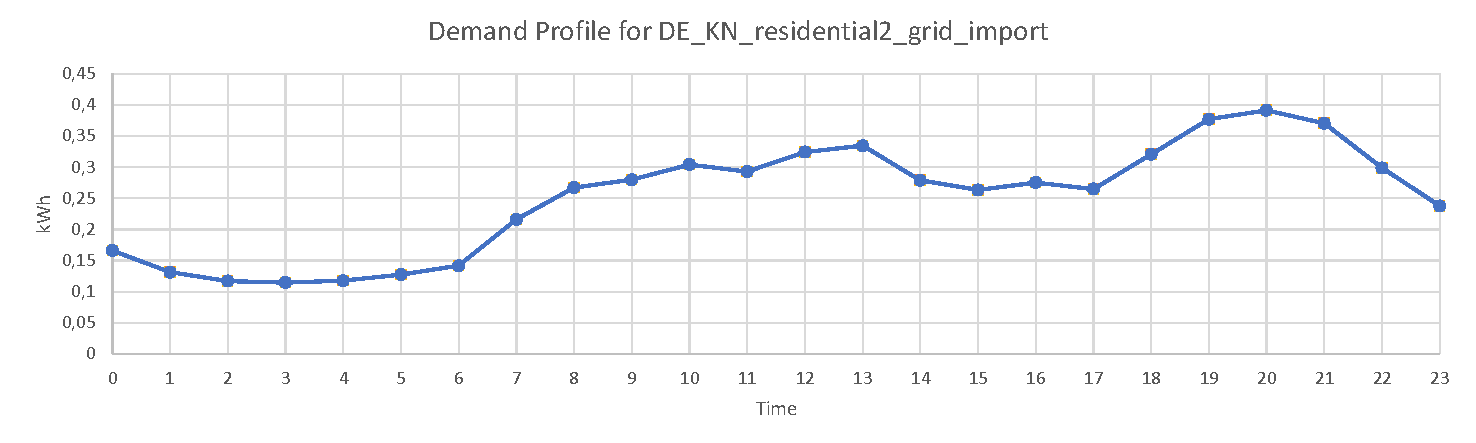
\includegraphics[width=1.00\textwidth]{../figures/profile1.pdf}
	\caption{Demand profile 1: Home building}
	\label{fig:profile1}
\end{figure}

\begin{figure}[!h]
	\centering
	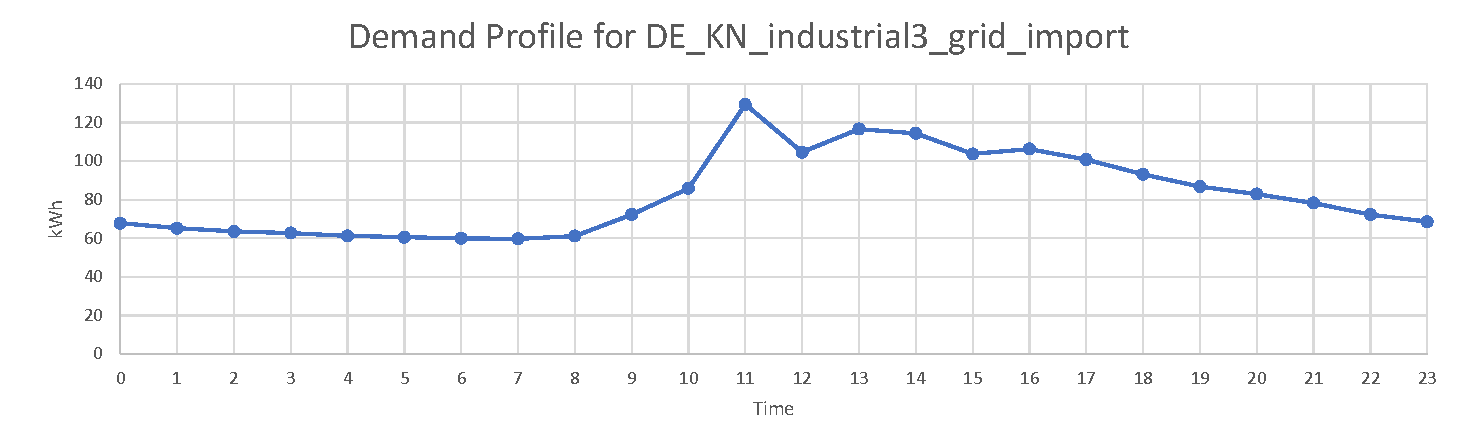
\includegraphics[width=1.00\textwidth]{../figures/profile2.pdf}
	\caption{Demand profile 2: Office building}
	\label{fig:profile2}
\end{figure}
